
%%%%%%%%%%% Nomenclature for this chapter%%%%%%%%%%
\nomenclature{TAU}{Tel-Aviv University}



\chapter{Basic examples}
\label{chap:chapter 1}




%%%%%%%%%%%%%%%%%%%%%%%%%%%%%%%%%%%%
%%%%%%%%%%%%%%%%%%%%%%%%%%%%%%%%%%%%

\section{Examples}
\label{sec:examples}


Citations are very simple. Add all the references in the references files.
You can you Google scholar to easily copy the bibtex.
For instance, this paper \cite{kour2014real} is awsome.

See Figure \ref{fig:figure_label} as an example on how to add figures to your thesis.
It is recommended that all figures to be kept in a separate directory.
Note the `./figures/figure' in the example below.


\begin{figure}
\centering
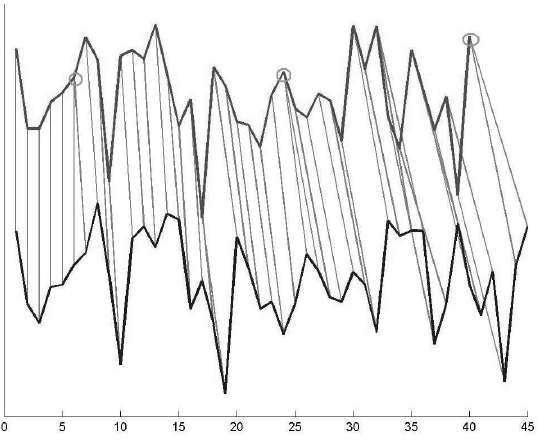
\includegraphics[width=0.5\textwidth]{./figures/figure}
\caption{A figure example.}
\label{fig:figure_label}
\end{figure}


See Table \ref{table:table_ex} to learn how to create tables.

\begin{table}
\centering
\caption{A table example}
\begin{tabular}{ c c c c }
\toprule
\textbf{Dataset} & \textbf{Number of samples} & \textbf{Results} & \textbf{Results 2} \\
\midrule                 
  Ini & 1405 & 48 & 9 \\ 
  Mid & 1196 & 52 & 10 \\ 
  Fin & 1629 & 44 & 9 \\ 
  Iso & 1372 & 39 & 8 \\ 
  \bottomrule
\end{tabular}
\label{table:table_ex} 
\end{table}

This how you create a new definition: go to \ref{def:distance_function}.

\begin{definition}
Given a data space $\mathfrak{D}$, for any two data elements $x,y \in \mathfrak{D}$, a \textbf{distance function} $dist$, on $\mathfrak{D}$ is defined as:
\begin{equation}
dist: \mathfrak{D} \times \mathfrak{D} \longrightarrow \mathds{R}_{\geq 0} 
\end{equation}
where $dist$ has the following properties:
\begin{compactitem}
\item $dist(x,y)=0 \Leftrightarrow x=y$ (reflexivity)
\item $dist(x,y) = dist(y,x)$ (symmetry)
\end{compactitem}
The pair $(\mathfrak{D},dist)$ is called a \textbf{distance space}.
\label{def:distance_function}
\end{definition}



\section {Nomenclature}

For updating nomenclature run the following commands:

makeindex Thesis-main.nlo -s nomencl.ist -o Thesis-main.nls

makeindex LettersClassification.nlo -s nomencl.ist -o LettersClassification.